\documentclass[11pt]{article}
\usepackage{fontspec}
\setmainfont{Arial}
\setsansfont{Arial}
\setmonofont{DejaVu Sans Mono}[Scale=MatchLowercase]
\usepackage[margin=1in]{geometry}
\usepackage{amsmath,amssymb}
\usepackage{graphicx}
\usepackage{booktabs}
\usepackage{array}
\usepackage{multirow}
\usepackage{siunitx}
\usepackage{caption}
\usepackage{subcaption}
\usepackage{placeins}
\usepackage{tikz}
\usetikzlibrary{arrows.meta,positioning,calc,fit,decorations.pathreplacing}
\usepackage[numbers,round]{natbib}
\usepackage[svgnames]{xcolor}
\usepackage{authblk}
\usepackage{microtype}
\usepackage{xurl}
\usepackage[hidelinks]{hyperref}

\captionsetup{font=small,labelfont=bf}
\setlength{\parskip}{0.3em plus 0.1em minus 0.05em}
\setlength{\parindent}{0pt}
\setlength{\emergencystretch}{1em}
\setlength{\textfloatsep}{10pt plus 3pt minus 3pt}
\setlength{\floatsep}{9pt plus 2pt minus 2pt}
\setlength{\intextsep}{9pt plus 2pt minus 2pt}
\renewcommand{\topfraction}{0.9}
\renewcommand{\bottomfraction}{0.85}
\renewcommand{\textfraction}{0.08}
\renewcommand{\floatpagefraction}{0.72}
\setcounter{topnumber}{3}
\setcounter{bottomnumber}{2}
\setcounter{totalnumber}{4}
\makeatletter
\setlength{\@fptop}{0pt}
\setlength{\@fpsep}{10pt plus 2pt}
\setlength{\@fpbot}{0pt plus 1fil}
\makeatother
\raggedbottom

\newcommand{\panfig}[1]{\resizebox{\textwidth}{!}{\input{#1}}}
\newcommand{\panhalffig}[1]{\resizebox{0.98\linewidth}{!}{\input{#1}}}

\graphicspath{{figures/}{standalone-assets/}{tikz/}{./}}
\newcommand{\InventoryFiles}{1587}
\newcommand{\LatentFiles}{1585}
\newcommand{\UniqueScores}{1236}
\newcommand{\NativeFiles}{910}
\newcommand{\NonNativeFiles}{675}
\newcommand{\ValidNativeFiles}{855}
\newcommand{\GuardedNativeFiles}{55}
\newcommand{\NullEligible}{60}
\newcommand{\NullCoherence}{59}
\newcommand{\NullJoint}{57}
\newcommand{\MaxExactDelta}{0.066412}

\hypersetup{pdftitle={Reference-anchored geometry diagnostics with noise-matched calibration and native-allocation checks},pdfauthor={Zeyu Fu}}
\title{\textbf{Reference-anchored geometry diagnostics with noise-matched calibration and native-allocation checks}}
\author[1]{Zeyu Fu}
\affil[1]{State Key Laboratory of Trauma and Chemical Poisoning, Institute of Combined Injury,
Chongqing Engineering Research Center for Nanomedicine, College of Preventive Medicine,
Army Medical University, Chongqing, China\\\texttt{fuzeyu09@gmail.com}}
\date{}
\begin{document}
\maketitle

\begin{abstract}
A structure-preservation score measures a specified relationship between objects; a high value does not certify a developmental trajectory. We audit that relationship using controlled coordinate interventions, explicit annotation inputs, and a versioned reference-anchored geometry battery (RAAG). A revised synthetic experiment uses the same initial jitter in faithful and damaged embeddings, three fixture seeds, and several perturbation severities. This removes a denoising confound in the historical shatter comparison. Local rank scores respond weakly to arm separation in this fixture, while reference-connected-pair survival reports the loss of connectivity. Official scIB trajectory conservation falls from 0.992--0.999 to 0.082--0.105 under shatter; the historical root-geodesic surrogate was misattributed to that API. RAAG v2 replaces a sampled Jensen--Shannon denominator with its exact distinct-pair mean and restricts quotable allocation coherence to native simplex outputs that pass degeneracy and dispersion guards. Re-scoring all \LatentFiles{} saved latent files in the frozen audit inventory requires \UniqueScores{} distinct computations: \ValidNativeFiles{} files have quotable native coherence, \GuardedNativeFiles{} are guarded, and \NonNativeFiles{} contain continuous coordinates. A focused permutation analysis reports its native denominator and retains all ten permutations per run. A further 444 fixed-object measurements examine graph scale, reference dimension, cell correspondence, and invariance controls. Across the tested scale grid, median within-object edge-survival range is 0.312; complete row reassignment reduces mean native coherence from 0.793 to 0.009 while reachability remains one. These are measurement and provenance results for fixed synthetic and stored computational objects, not evidence that a model recovered biological branches.
\end{abstract}

\section{Introduction}

Low-dimensional representations are routinely used to summarize single-cell expression data, compare cell populations, and display gradual changes between transcriptional states. Their apparent simplicity creates a demanding measurement problem. A visually continuous path, a compact labelled group, and a probability vector that changes smoothly between neighbouring cells describe different properties. Each can be useful, yet none alone identifies the biological process that produced the observations. Evaluation therefore needs to specify both the object being measured and the relationship against which preservation is assessed. This study examines how that specification changes the interpretation of geometric scores through controlled coordinate interventions and remeasurement of fixed computational objects.

Neighbourhood preservation has a well-developed methodological basis. Trustworthiness and continuity assess intrusions and omissions in local neighbourhood rankings~\cite{venna2006local,venna2010retrieval}. Co-ranking summaries express related relationships across neighbourhood scales~\cite{lee2009quality}. These approaches make locality explicit, which is valuable when nearby observations should remain nearby after projection. However, a question about the fate of a reference-connected pair is distinct from a question about the rank of an immediate neighbour. A small number of changed edges can separate large graph components while affecting relatively few local comparisons. The magnitude of that response is an empirical property of the graph and intervention, rather than a universal defect of a metric family.

Other evaluation traditions address complementary structures. Geodesic approaches use graph paths to represent relationships beyond immediate neighbours~\cite{tenenbaum2000global}, while inter-cluster reliability diagnostics examine changes in cluster organization~\cite{jeon2022steadiness}. In single-cell integration, evaluation also includes preservation of supplied biological annotations and trajectory-related ordering~\cite{luecken2022benchmarking}. Trajectory benchmarks distinguish topology, ordering and feature recovery as separate targets~\cite{saelens2019comparison}. Those annotations add information unavailable to a purely coordinate-based diagnostic. They also change the estimand: connectedness within a labelled group need not measure connectedness between groups, and agreement with an inferred ordering need not establish a biological lineage. A comparison is interpretable only when the graph construction, annotation inputs, and implementation identity are reported together with the score.

Calibration by controlled damage offers a direct way to investigate these distinctions. Starting from the same reference, one can separate two arms, compress a branching coordinate, add noise, or break row correspondence while preserving the candidate marginal distribution. The intended intervention must nevertheless be isolated from incidental changes. If a damaged candidate removes the noise present in its comparator, an apparently favourable local response can combine denoising with structural damage. Likewise, a named software API and a locally implemented surrogate can behave differently even when both are described informally as trajectory conservation. Matched starting coordinates and direct upstream execution are therefore essential parts of a measurement experiment.

Probability-valued representations introduce an additional object-identity requirement. A native allocation vector assigns mass across defined coordinates of a model; an arbitrary continuous embedding does not become such an allocation merely because softmax makes its rows sum to one. For native allocations, Jensen--Shannon divergence~\cite{lin1991divergence} provides a bounded comparison between probability vectors. A smoothness ratio can compare divergence on reference edges with divergence among all cells, but its denominator determines the meaning and reproducibility of the result. Sampling positional pairs can introduce dependence on row order. Nearly uniform or constant allocations can also make a favourable ratio uninformative about useful between-cell variation.

Reference-anchored allocation geometry, abbreviated RAAG, addresses these questions with separately reported diagnostics. Reachability measures whether reference-connected pairs remain connected. Edge survival measures the hop distance between reference neighbours, and separation survival asks whether distant reference pairs remain separated relative to a candidate threshold. Allocation coherence compares local and overall probability variation only when native allocation semantics and operational dispersion checks are satisfied. Keeping these quantities separate makes their different failure responses visible. Their common reference is a declared expression representation, not an assertion that the reference graph is biological ground truth or that all its features should necessarily be preserved.

We evaluate this measurement design in two complementary settings. A small branching fixture supplies exact coordinate interventions, common initial noise, and explicit branch and pseudotime annotations for official metric calls. A frozen inventory of saved representations supplies heterogeneous real-data computational objects whose identities, duplicate aliases, and allocation semantics can be traced. We then extend the analysis using a fixed subset to vary graph neighbourhood size, retained reference dimension, and the fraction of corrupted cell correspondences. These choices probe sensitivity within the observed inputs; they do not create new patients or independent biological experiments. All intervention levels and object-selection rules are fixed before computing the new sensitivity results.

The study asks what evidence is needed before a geometric measurement can support a stated interpretation. Its design examines noise matching, the identity of official and surrogate trajectory implementations, exact distinct-pair normalization, and the eligibility of allocation-valued inputs. Sensitivity to reference construction and cell correspondence provides a further test of the measurement design. The intended use is to diagnose specified geometric relationships and expose interpretations that the chosen inputs cannot justify. Evidence about observed lineage, prospective cell fate, or generalization to a new biological cohort would require additional measurements with those targets explicitly defined.

\section{Materials and Methods}

\subsection{Measurement workflow and analysis objects}

Figure~\ref{fig:workflow} separates the coordinate and native-allocation pathways. The coordinate input is a finite matrix $Z\in\mathbb R^{n\times q}$ paired row-for-row with a reference $X\in\mathbb R^{n\times d}$. The allocation pathway additionally requires model-declared probabilities $P\in\Delta^{K-1}$ for each cell; numeric normalization alone cannot supply that interpretation. Graph scores, allocation eligibility, dispersion and null comparisons remain separate outputs. No combined biological-success score is constructed. Preprocessing and the chosen reference define the question being asked, as they do elsewhere in single-cell analysis~\cite{luecken2019practices}.

\begin{figure}[!htbp]
\centering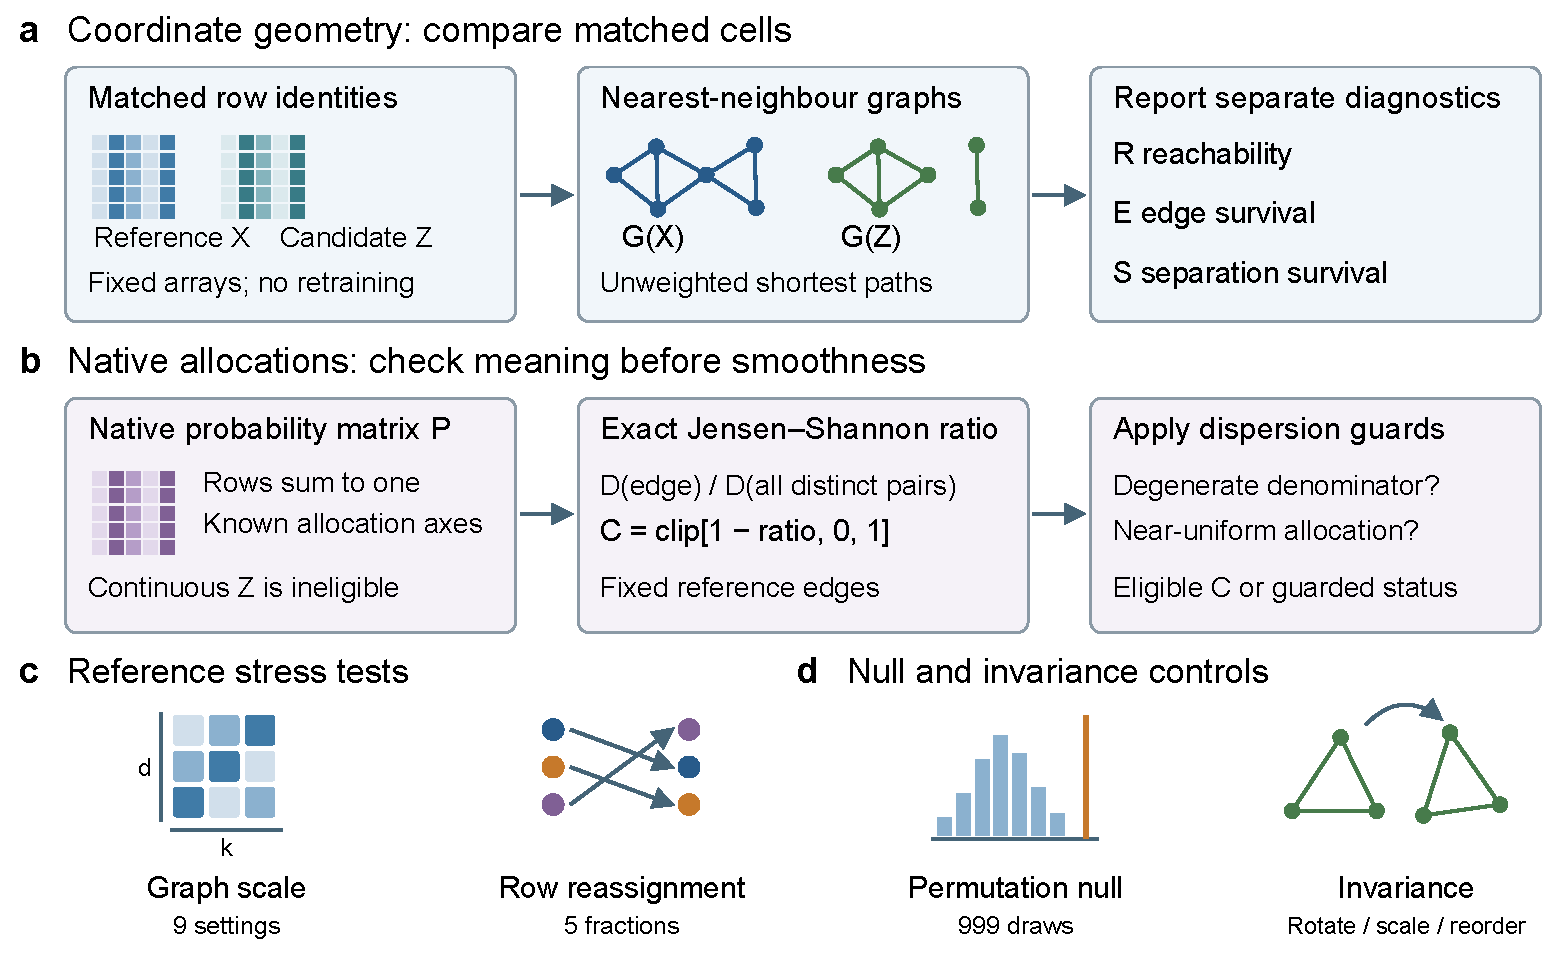
\includegraphics[width=\linewidth]{figures/architecture.pdf}
\caption{Measurement modules and the routes through them. A: matched reference and candidate rows generate separate undirected nearest-neighbour graphs; shortest paths supply reachability $R$, edge survival $E$ and separation $S$. B: a model-declared native probability matrix supplies Jensen--Shannon divergences on reference edges and over all distinct pairs; denominator and dispersion guards determine whether coherence is quotable. Continuous coordinates stop before this pathway. C: graph settings, row reassignment, null draws and invariance checks probe fixed computational objects. Matrices and graph nodes are illustrative, not data or inferred biological modules.}
\label{fig:workflow}
\end{figure}

\subsection{Reference-anchored geometry}

Let $X=(x_i)_{i=1}^n$ be the reference and $Z=(z_i)_{i=1}^n$ the candidate, with the same cell identity in each row. On each space we construct the undirected union of a Euclidean $k$-nearest-neighbour graph, using $k=15$. Let $h_X(i,j)$ and $h_Z(i,j)$ denote unweighted shortest-path distances, with infinity for disconnected pairs. Let $\mathcal P_X=\{(i,j):i<j,\ h_X(i,j)<\infty\}$ and let $E_X$ be the undirected reference edges. Reachability and edge survival are
\begin{align}
 R(X,Z)&=\frac{1}{|\mathcal P_X|}\sum_{(i,j)\in\mathcal P_X}\mathbf 1[h_Z(i,j)<\infty],\\
 E(X,Z)&=\frac{1}{|E_X|}\sum_{(i,j)\in E_X}\frac{1}{h_Z(i,j)},\qquad 1/\infty=0.
\end{align}
The first counts connected pairs; the second measures local adjacency distortion. A small number of severed junction edges can disconnect many pairs. Conversely, a connected but randomly reordered candidate can have $R=1$, so $R$ alone is not a quality score. Neighbours use Euclidean distance, the union rather than intersection of directed neighbour lists, and $k'=\min(\max(k,1),n-1)$. Graph edges carry unit weight. Each unordered pair or edge enters its denominator once; the score formulas exclude self-pairs. The archived neighbour constructor drops the first returned rank, assuming it is the query itself. Exact duplicates can violate this assumption; the tie stress test below therefore delimits this implementation. Nonfinite inputs and reference populations with fewer than ten connected pairs are rejected instead of receiving a favourable score.

For separation survival, the reference far set $F_X$ contains finite reference pairs at or above the 90th percentile of $h_X$. Let $m_Z$ be the median finite candidate hop distance. We define
\begin{equation}
 S(X,Z)=\frac{1}{|F_X|}\sum_{(i,j)\in F_X}\mathbf 1[h_Z(i,j)\geq m_Z].
\end{equation}
Disconnected candidate pairs count as separated. This convention is complementary to reachability, but the candidate-dependent threshold also limits interpretation: $S$ is not an absolute distance-preservation measure. Graph construction, tied distances, $k$, and the chosen reference can change the answer. The baseline setting is $k=15$ with a 50-component reference. The additional sensitivity experiment varies $k$ and the retained reference dimension explicitly, over a finite grid described below.

\subsection{Exact coherence and applicability}

Allocation coherence requires a native allocation matrix $P$ with rows $p_i\in\Delta^{K-1}$ representing probabilities over the model's allocation coordinates. The Jensen--Shannon divergence~\cite{lin1991divergence} is computed in natural-log units after the implementation's fixed $10^{-12}$ clipping and row renormalization. Define
\begin{align}
 D_E &= |E_X|^{-1}\sum_{(i,j)\in E_X}\operatorname{JSD}(p_i,p_j),\\
 D_{\rm all} &= {\binom n2}^{-1}\sum_{i<j}\operatorname{JSD}(p_i,p_j),\\
 C_{\rm raw} &= \left[1-D_E/D_{\rm all}\right]_0^1.
\end{align}
For two allocation rows, $\operatorname{JSD}(p,q)=\tfrac12\sum_jp_j\log(p_j/m_j)+\tfrac12\sum_jq_j\log(q_j/m_j)$ with $m=(p+q)/2$. RAAG v2 uses every unordered distinct pair in $D_{\rm all}$. The historical implementation sampled positional pairs using a fixed seed. Jointly reordering reference and allocation rows therefore changed the sampled denominator even though the scientific object was unchanged. Exact summation removes this sampling dependence, up to floating-point accumulation, at $O(n^2K)$ arithmetic cost. The implementation uses bounded row-block memory for the denominator; all-pairs graph distances still require quadratic storage. Unit tests compare the denominator with independently enumerated SciPy Jensen--Shannon distances and test joint row reordering.

The mean row perplexity is $\bar P=n^{-1}\sum_i\exp[-\sum_kp_{ik}\log p_{ik}]$. A denominator at or below $10^{-12}$ yields status \texttt{degenerate}; $\bar P/K>0.95$ yields \texttt{near\_uniform}. Neither produces a quotable coherence value; the degenerate raw diagnostic is set to zero by convention. A constant uniform matrix satisfies both flags; the status gives degeneracy precedence. The thresholds are declared operational guards, not estimated biological decision boundaries. Raw diagnostics remain available for auditing.

Continuous Gaussian coordinates receive status \texttt{non\_native}. Softmax of these coordinates is reported only under \texttt{softmax\_coordinate} fields. Its dimension is the number of latent coordinates, which is 10 for the stored mixture-regularized representations, not their mixture truncation of 50. This transformation is not a posterior responsibility matrix and cannot support allocation claims. Numerical simplex inference is available for backwards-compatible calls, but the inventory and all reported re-scores pass an explicit semantic declaration.



\subsection{Matched-noise calibration and upstream identity}

The synthetic reference contains 450 points in two dimensions: a 150-point trunk and two 150-point arms. Reference coordinates include independent Gaussian noise with standard deviation 0.004. A faithful candidate adds noise with standard deviation 0.01 and is therefore not an isometric copy of the reference. Every revised damage intervention begins with that same faithful realization. We translate the two arms by opposing vertical shifts of 0.5, 2.5, or 9; retain 0.5 or 0 of the fork coordinate for collapse; add noise of standard deviation 0.06 or 0.18; or permute candidate rows. Identity and a rotation/uniform rescaling of faithful provide controls. Seeds 7, 17, and 42 each yield 12 candidates, including the historical unmatched shatter as a separately named diagnostic. As in the locked fixture, reference and faithful jitter generators share the fixture seed, so their initial draws are coupled; the three seeds are paired fixture realizations, not independent biological samples. The protocol was written before this new sweep; its design follows discovery of the old confound and is not a prospective confirmatory registration.

We run the historical LSE/LSEX/DRE measurement implementation, canonical local-rank and graph metrics, zadu implementations including steadiness and cohesiveness, and RAAG. Official scIB 1.1.7 is called directly through both public APIs~\cite{scib2026api}. Scanpy~\cite{wolf2018scanpy} constructs the candidate neighbour graph from \texttt{X\_emb}, with \texttt{n\_neighbors=15}. Synthetic branch labels and known pseudotime are supplied in \texttt{obs}; the trajectory API computes diffusion pseudotime internally~\cite{haghverdi2016diffusion}. There is no batch covariate. This is an explicit synthetic stress test of those API inputs, not a complete integration benchmark.

The local root-geodesic surrogate correlates reference and candidate root distances on reachable rows; official scIB uses diffusion pseudotime and its own component/root handling. The two computations are assigned distinct identifiers throughout the measurement record. Every stack result retains warnings, exceptions, or nonfinite status. Failed official calls are never replaced by the surrogate.



\subsection{Historical inventory and permutation comparison}

The inventory includes all NPZ files in a frozen historical computational evidence collection. It finds \InventoryFiles{} files, including \LatentFiles{} latent arrays with valid stored test indices and two non-latent containers. Computation identity includes dataset, test-index bytes, latent bytes, and semantic allocation type. This retains every file alias while reducing scoring to \UniqueScores{} distinct objects. Smoke runs and probes remain tagged; neither aliases nor repeated checkpoints are treated as independent observations. Aggregate results without a saved latent array in this collection are outside the re-score coverage.

Four historical expression caches are loaded only after their SHA256 values match the stored input contracts. The reconstructed normalized matrix, cast to the historical float64 hashing convention, must also match its original digest. PCA with 50 components and seed 42 is fitted on the actual stored test indices, producing 14 dataset/index reference objects. This reproduces the historical, transductive expression-reference estimand; it does not turn the old preprocessing into training-only preprocessing. The stored backgrounds are hematopoiesis~\cite{setty2019palantir}, dentate gyrus~\cite{hochgerner2018conserved}, pancreatic endocrinogenesis~\cite{bastidas2019endocrinogenesis}, and adult lung tissue~\cite{vieirabraga2019lung}. The Lung accession GSE130148 originates from four adult patients~\cite{lung_geo130148}; the historical cell-random splits are not patient holdouts. Organ annotations and inferred fate probabilities have different provenance from biological ground truth.

For the historical focused 144-run manifest we retain every run and ten row permutations per run, using seed 0. A permutation preserves the latent marginal distribution while destroying correspondence to reference rows. We report whether the observed score exceeds the maximum of those ten values. This is descriptive: the smallest Monte Carlo permutation $p$-value with the observed arrangement included is $1/11\approx0.091$~\cite{phipson2010permutation}. These comparisons do not establish 5\% significance, and native coherence uses only eligible native rows.


\subsection{Frozen scale and correspondence experiments}

A protocol fixed selection, settings, corruption seeds, and output quantities before the new sensitivity computations. The selected representations use the same four backgrounds, stored seeds 0, 1, and 2, and ten coordinates. Native objects were trained under a symmetric concentration-one allocation prior; continuous objects used a mixture penalty of weight one with truncation 50. They are selected by these configuration names, without inspecting their new scores. Their role here is to supply probability-valued and continuous computational objects, not to estimate a difference in model effectiveness. The local input manifest preserves original file identity, byte hashes, matched test indices, and the full selected latent/reference arrays.

For graph sensitivity, each object is scored at all nine combinations of three neighbour counts and three retained reference ranks. For correspondence sensitivity, a seeded permutation chooses a nested subset of $\lfloor fn\rfloor$ cells at each fraction $f\in\{0,0.1,0.25,0.5,1\}$. Their allocation rows are reassigned in a single cycle. Fractions select nested sets, but their cycle assignments differ. Corruption seeds are 0, 17, and 42; the exact changed fractions are recorded. The allocation marginal distribution is unchanged, and the reference is fixed. Geometry and applicable exact coherence are recomputed after each intervention.

A subsequent, separately declared paired-grid audit subtracts the continuous-coordinate score from the native-allocation score for each background--seed pair at every one of the nine $k/d$ settings. We record strict sign reversals relative to $(k,d)=(15,50)$, exact ties, and within-pair difference ranges for reachability, edge survival, and separation. The twelve pairs are selected computational objects, not donors or a randomized comparison of methods; unlike the within-object scale analysis, their candidate representations also differ in model, training, and semantic type. These contrasts test whether a descriptive ordering is sensitive to the measurement setting, not which model is superior.

Separately from the historical 144-run comparison with ten permutations, a new fixed-object analysis tests exactly twelve eligible native arrays at the baseline setting. For each, it holds the reference graph and allocation-row multiset fixed, generates 999 independent random row orders with a recorded PCG64 seed reset per object, and reassigns allocation rows before computing exact coherence. Precomputed pairwise Jensen--Shannon distances preserve the all-distinct-pair denominator. The unpermuted score is checked against the frozen battery to $10^{-12}$. With null ties counted against the observed score, the one-sided Monte Carlo probability is $(1+\#\{C_{\rm null}\geq C_{\rm observed}\})/1000$. This tests row correspondence under that exchangeability null, not a population-level biological hypothesis; no across-object multiplicity claim is made.

The invariance controls use one fixed orthogonal transform followed by scaling by 2.5, and one fixed joint row permutation per object. Geometry uses the rotated continuous coordinates directly; allocation coherence is not interpreted for the rotated arrays. Joint row permutation retains the original semantic declaration. All 444 batteries run on CPU with at most two numerical threads and no optimizer updates. Complete rows, unavailable values, input hashes, scorer and driver hashes, protocol identity, and elapsed execution time are retained. Summaries are descriptive; neither the grid settings nor the corrupted copies are treated as independent experimental units.

\subsection{Independent recomputation and statistical scope}

A post hoc robustness audit recomputes the 216 graph-grid results without importing the archived scorer. It explicitly removes self-distances, sorts pair distances, forms union graphs and computes shortest paths in a separate SciPy implementation. Exact ties at the neighbour cutoff are counted because they can make neighbour identity depend on tie handling. Native coherence is independently evaluated from a full Jensen--Shannon matrix; its constant distinct-pair denominator allows fast permutation of row indices. We reproduce the archived 999-draw stream and run a second stream with seed 104729, reinitialized separately for each of the twelve native objects. Each stream retains its own $(b+1)/(999+1)$ probability, with $b$ counting null scores greater than or equal to the observed score~\cite{phipson2010permutation}; streams are not retrospectively pooled.

The audit also reports a post hoc Holm correction for the twelve original fixed-object probabilities~\cite{holm1979sequential}. For sorted probabilities $p_{(i)}$, the adjusted value is $\min\{1,\max_{j\leq i}(12-j+1)p_{(j)}\}$. This family is limited to the twelve baseline native-coherence tests, excluding other metrics and the separate historical 144-run inventory. Such correction addresses this declared multiplicity, not exchangeability of donors, selection of datasets or population generalization. The same saved cells, graph settings and algorithmic seeds cannot provide independent biological replication~\cite{zimmerman2021pseudoreplication}.

An additional synthetic stress test deliberately violates the no-tie setting: twenty candidate rows have the same three-dimensional zero coordinate, paired with Gaussian reference rows generated with seed 91. At $k=5$ we count self-loops and jointly reorder both matrices with seeds 0, 17 and 42. This probes exact coordinate collapse; it is separate from the 24 stored objects and does not silently replace their frozen scorer or results.

\section{Results}

The measurement quantities operate on different input relationships, summarized in Table~\ref{tab:estimands}. The comparison preserves the distinction between coordinate diagnostics, native probability allocations, and metrics that require supplied annotations. An earlier root-geodesic surrogate was labelled as official scIB trajectory conservation; direct implementation comparison identifies that attribution error, which is corrected throughout this study.

\begin{table}[htbp]
\centering\small
\begin{tabular}{>{\raggedright\arraybackslash}p{0.25\linewidth}>{\raggedright\arraybackslash}p{0.31\linewidth}>{\raggedright\arraybackslash}p{0.34\linewidth}}
\toprule
Quantity & Input relationship & Permitted interpretation\\
\midrule
RAAG $R,E,S$ & Matched candidate/reference rows & Coordinate graph preservation relative to that reference\\
Native coherence & Reference edges and native simplex probabilities & Allocation smoothness relative to nonlocal allocation variation\\
Local root surrogate & Reference and candidate root distances on reachable rows & Conditional rank agreement of graph distances\\
Official scIB connectivity & Candidate graph and supplied branch labels & Within-label connectedness\\
Official scIB trajectory & Known pseudotime, labels, candidate graph & Conservation of an annotation-derived ordering by diffusion pseudotime\\
\bottomrule
\end{tabular}
\caption{Measurement objects and scope. No entry alone identifies biological lineage truth. The local surrogate and official scIB trajectory metric are distinct computations.}
\label{tab:estimands}
\end{table}

\subsection{A matched intervention changes the interpretation}

\begin{figure}[htbp]
\centering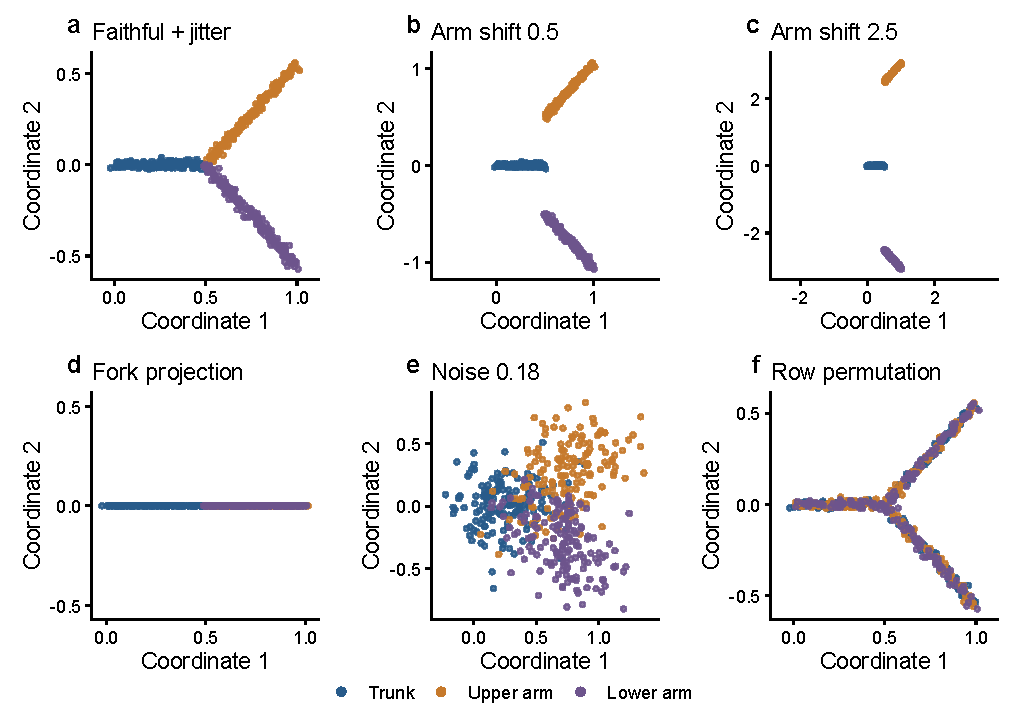
\includegraphics[width=\linewidth,height=0.64\textheight,keepaspectratio]{calibration_perturbations.pdf}
\caption{Matched-noise coordinate interventions for fixture seed 42. Row A shows the faithful candidate and opposing arm translations of 0.5 and 2.5, from left to right. Row B shows removal of the fork coordinate, additional Gaussian noise with standard deviation 0.18, and permutation of candidate rows. Each view retains all 450 cells: 150 trunk cells and 150 in each arm. The shared colour key between rows identifies these original branch labels in every view, including after permutation. All damaged candidates start from the same faithful jitter realization, so the comparison does not remove baseline noise. Axes show candidate coordinates with independently chosen ranges and equal coordinate aspect within each view; absolute separation should therefore be read from the axis values. Row permutation changes coordinate-to-cell correspondence while retaining label values and the marginal coordinate distribution. These are synthetic interventions, not observed biological trajectories.}
\label{fig:interventions}
\end{figure}

Figure~\ref{fig:interventions} documents the intervention itself. Table~\ref{tab:calibration} gives the seed-42 scores, while Figure~\ref{fig:response} displays all three seeds and shatter amplitudes. The full machine-readable record includes all 36 candidates and all metric stacks. Differences across these seeds describe fixture repeatability, not biological replication or statistical power.

The historical seed-42 shatter was constructed from the reference instead of the faithful candidate. Its trustworthiness was 0.999353 versus 0.997404 for faithful; edge survival was 0.974531 versus 0.921448. Matching the faithful noise changes the shatter values to 0.997025 and 0.906474, respectively. The trustworthiness response is small, but its sign is no longer an improvement. Reachability is 0.331849 under either construction. Thus the historical sign reversal was partly a noise confound. The large contrast between local and pair-connectivity sensitivity remains a fixture-specific observation, rather than a proof that local scores never respond to tearing.

\begin{table}[htbp]
\centering\small
\begin{tabular}{lrrrr}
\toprule
Metric & Faithful & Shatter & Collapse & Permuted \\
\midrule
Trustworthiness & 0.9974 & 0.9970 & 0.7997 & 0.5084 \\
LCMC (zadu) & 0.7718 & 0.7685 & 0.4924 & 0.0011 \\
Local root-geodesic surrogate & 0.9997 & 0.9983 & 0.9994 & 0.4850 \\
scIB graph connectivity & 1.0000 & 1.0000 & 0.9200 & 0.4378 \\
scIB trajectory conservation & 0.9943 & 0.0960 & 0.5272 & 0.5114 \\
RAAG reachability & 1.0000 & 0.3318 & 1.0000 & 1.0000 \\
RAAG edge survival & 0.9214 & 0.9065 & 0.7456 & 0.1465 \\
RAAG separation & 1.0000 & 1.0000 & 0.6952 & 0.5357 \\
\bottomrule
\end{tabular}

\caption{Seed-42 calibration, with matched noise and $k=15$. Shatter uses amplitude 2.5; collapse retains zero fork coordinate. Values come directly from the named implementation. NA denotes an explicitly retained unavailable or nonfinite result. The official trajectory row must not be identified with the local surrogate.}
\label{tab:calibration}
\end{table}

\begin{figure}[htbp]
\centering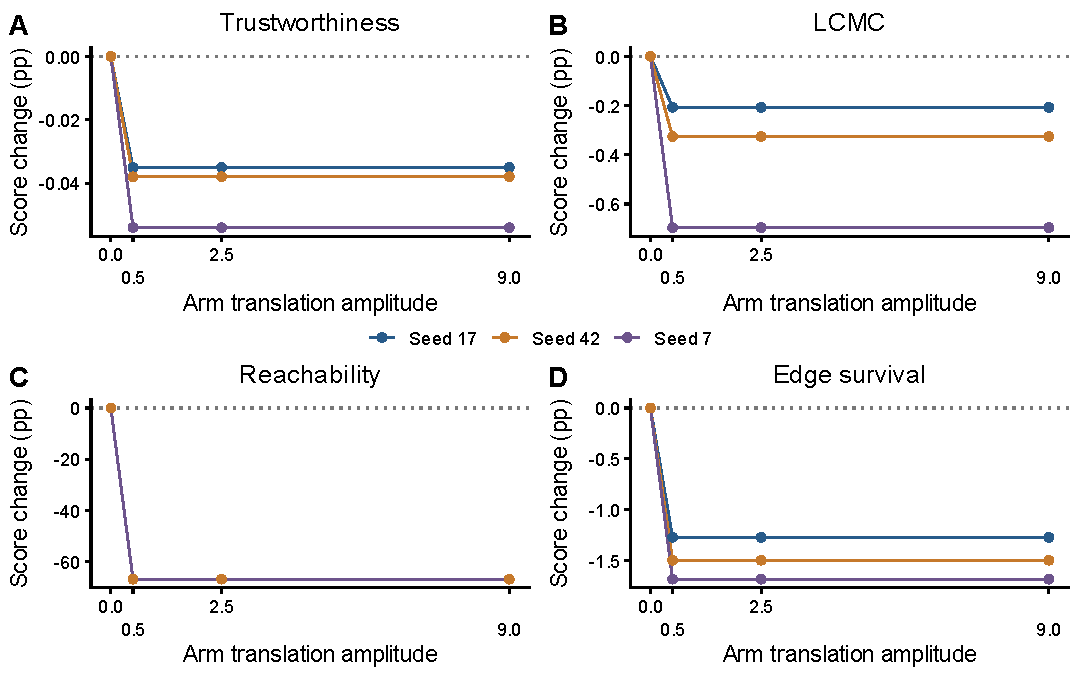
\includegraphics[width=\linewidth,height=0.64\textheight,keepaspectratio]{graph_disconnection_response.pdf}
\caption{Metric responses to opposing arm translations with matched baseline noise. Panels A--D show trustworthiness, local continuity meta-criterion (LCMC), reference-connected-pair reachability, and reference-edge survival, respectively. Each coloured line follows one of the same three fixture seeds, 7, 17, and 42; a single colour key between the rows applies to all four panels. Points show the four tested translation amplitudes, 0, 0.5, 2.5, and 9, on the horizontal axis. Amplitude zero is the faithful candidate, and the vertical value is 100 times the difference from that seed's faithful score, expressed in percentage points. The dotted zero line marks no change. Vertical ranges differ to retain small local responses; connecting lines guide the eye and do not represent a continuous sweep. The paired fixture realizations are not biological samples, and no detection threshold or minimum useful effect is inferred.}
\label{fig:response}
\end{figure}

Official graph connectivity conditions on branch labels, so it can remain high when the labelled arms are individually connected but disconnected from one another. That is compatible with its definition. A high root-order correlation can likewise coexist with changed branch geometry. The official trajectory score falls from 0.9917--0.9986 for faithful to 0.0816--0.1046 for matched shatter across the three seeds; collapse scores 0.5272--0.5595. This directly contradicts the earlier claim of scIB shatter-blindness. Its identity-control score is only 0.3836--0.3902, showing that the API's root/diffusion procedure is also sensitive to this particular fixture. We report these observations without replacing them with a preferred surrogate or claiming that they characterize all integration settings. Collapse and noise responses also vary across the tested severities; the earlier binary figure's direction labels and universal failure wording are removed.

\subsection{Exact allocation coherence needs guards and identity}

Figure~\ref{fig:allocation} separates raw coherence from perplexity. A smooth near-uniform allocation can have high raw coherence because both numerator and denominator are small. The guard withholds the quotable score. A constant allocation has no between-cell contrast; a uniform constant is also near-uniform. Sharp rows can be coherent or incoherent depending on their correspondence to the reference. Neither smoothness nor sharpness alone certifies a useful allocation.

\begin{figure}[htbp]
\centering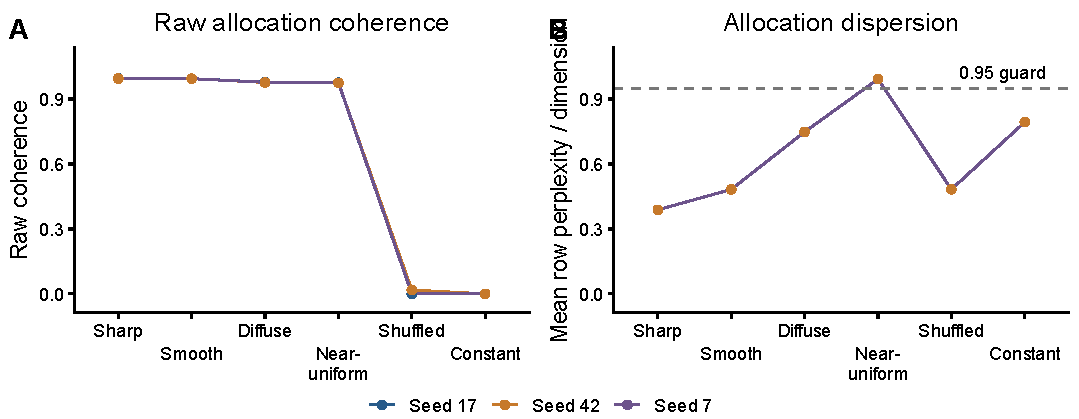
\includegraphics[width=\linewidth,height=0.64\textheight,keepaspectratio]{allocation_validity_guards.pdf}
\caption{Native-allocation diagnostics across the declared allocation ladder. Panel A shows raw allocation coherence, including diagnostic values that are not eligible for quotation as native coherence. Panel B shows mean row perplexity divided by the actual simplex dimension, so a value near one indicates broadly dispersed allocations. Categories run from sharp, smooth, and diffuse allocations through near-uniform, shuffled, and constant controls. Each coloured line retains one fixture seed, 7, 17, or 42; the shared horizontal key applies to both panels, and lines connect discrete controls rather than a calibrated continuous dose. The dashed 0.95 line marks the operational near-uniform guard in B. Constant allocations are guarded for degeneracy regardless of perplexity; their zero raw coherence is an implementation convention, not measured evidence of complete biological incoherence. The three seeds describe synthetic fixtures and do not supply population-level uncertainty.}
\label{fig:allocation}
\end{figure}

Across the historical inventory, \NativeFiles{} files contain native allocations: \ValidNativeFiles{} are quotable and \GuardedNativeFiles{} are guarded. The remaining \NonNativeFiles{} contain continuous coordinates. Among the 804 distinct native objects, the largest absolute change from the re-executed historical sampled estimator is \MaxExactDelta{}. The mean signed change is 0.000606. Exact replacement therefore cannot be characterized as a machine-precision-only revision. Geometry definitions are unchanged. All \UniqueScores{} computations completed; the two excluded NPZ containers remain listed rather than silently dropped.

\subsection{A denominator correction to the real-data null statement}

The focused historical manifest contains 60 native simplex allocations and 84 outputs with continuous coordinates. The latter comprise 48 mixture-regularized and 36 Gaussian variational controls. The old count of 142/144 coherence values above the null maximum combined these incompatible objects; 140/144 passed its joint comparison of edge survival, separation, and coherence. The exact scorer reports \NullEligible{} quotable native allocations, of which \NullCoherence{} exceed all ten coherence permutations and \NullJoint{} exceed the edge, separation, and coherence maxima jointly (Figure~\ref{fig:coverage}). There are no near-uniform native rows in this focused manifest, so the near-uniform guard does not explain the denominator correction. Allocation identity explains that population correction; replacing the sampled denominator additionally changes the native above-null count from the historical 58/60 to 59/60 and the joint count from 56/60 to 57/60. The complete inventory does contain guarded native outputs; these are a different population.

\begin{figure}[htbp]
\centering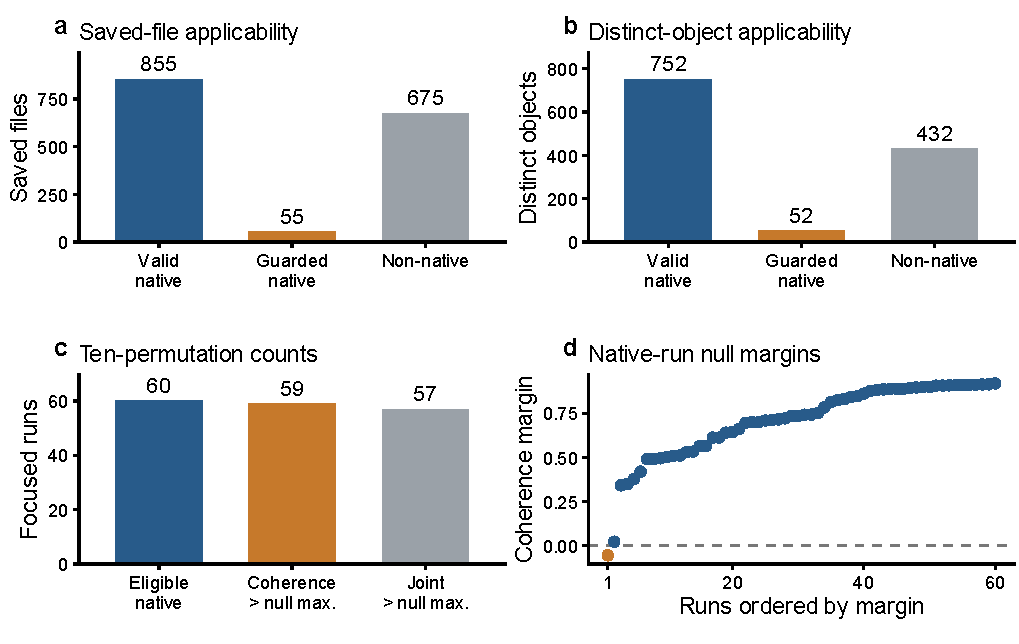
\includegraphics[width=\linewidth,height=0.64\textheight,keepaspectratio]{inventory_null_comparison.pdf}
\caption{Applicability and permutation comparisons with explicitly different denominators. Panel A counts all \LatentFiles{} saved latent files in the frozen inventory, including retained aliases: valid native allocations, native allocations guarded for near-uniformity or degeneracy, and non-native continuous coordinates. Panel B concerns the separate focused manifest of 144 runs. Its bars count eligible native runs, those whose coherence exceeds the maximum of their ten row-permuted values, and those exceeding that maximum jointly for edge survival, separation, and coherence. Horizontal position and the black annotation give each descriptive count; bar colours distinguish the labelled categories within each panel and do not define a common category scale across populations. Exceeding all ten permutations does not establish 5\% Monte Carlo significance, since the smallest corrected permutation probability is $1/11$. Repeated files, seeds, and checkpoints are not independent biological units.}
\label{fig:coverage}
\end{figure}


\subsection{Dependence on graph scale and reference dimension}

The fixed sensitivity subset contains 24 computational objects: a native allocation and a continuous-coordinate representation for each of four backgrounds and three stored seeds. All nine combinations of $k\in\{5,15,30\}$ and reference dimension $d\in\{10,25,50\}$ are evaluated, giving 216 complete batteries. Figure~\ref{fig:scale} displays deviations from each object's $k=15,d=50$ baseline, averaged across its three stored seeds. The candidate arrays are unchanged throughout this experiment.

\begin{figure}[htbp]
\centering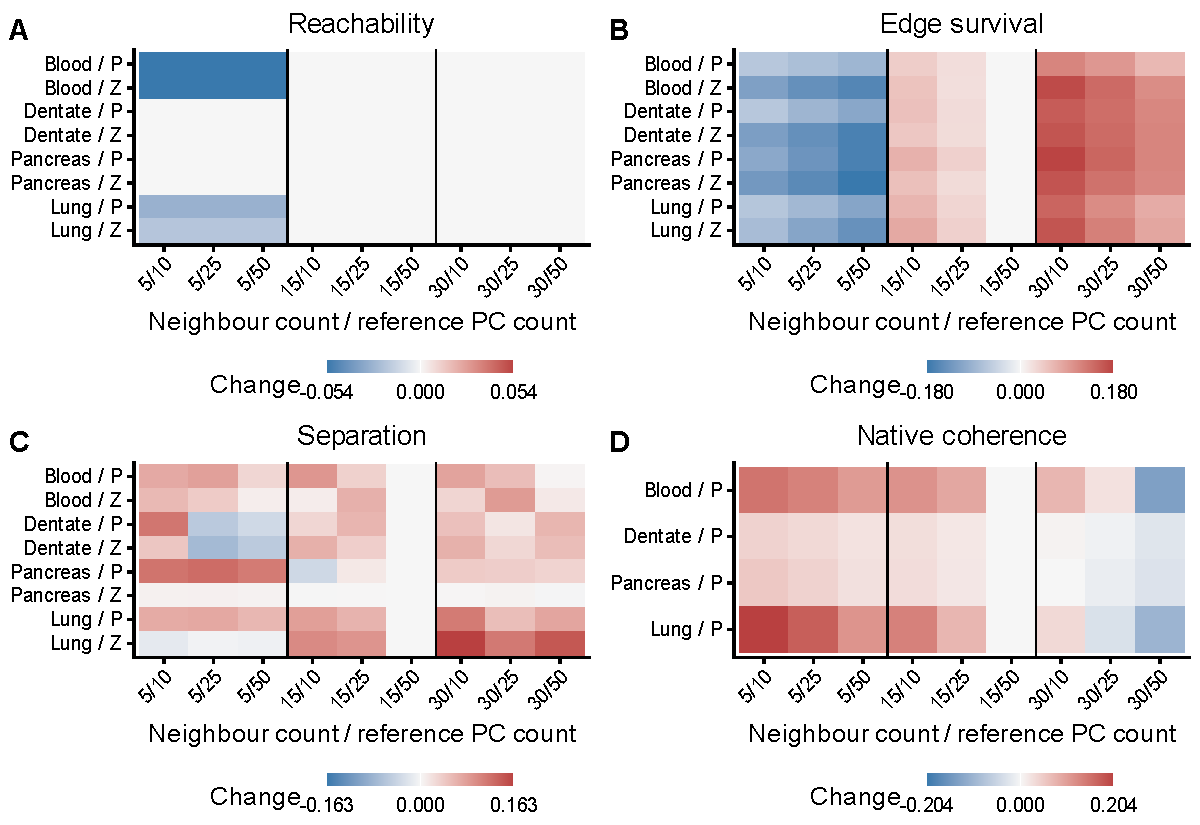
\includegraphics[width=\linewidth,height=0.64\textheight,keepaspectratio]{scale_reference_sensitivity.pdf}
\caption{Sensitivity to graph scale and retained reference dimension for fixed candidate arrays. Panels A--D show reachability, edge survival, separation, and native coherence, respectively. Columns enumerate the nine combinations of neighbour count $k\in\{5,15,30\}$ and reference PC count $d\in\{10,25,50\}$; vertical rules separate neighbour-count groups. Rows identify blood, dentate gyrus, pancreatic endocrinogenesis, and lung backgrounds, with P denoting native probabilities and Z continuous coordinates. Each tile is the mean change across three stored seeds from those same objects' $k=15,d=50$ setting. Panel D includes native objects only. Each metric retains its own symmetric colour scale, centred on zero, because the observed numerical ranges differ; colours cannot be compared quantitatively between panels. Positive and negative values indicate direction, not preferred settings. The 10- and 25-PC references truncate the existing 50-PC reference without refitting PCA. The four backgrounds and repeated settings are not biological replication units.}
\label{fig:scale}
\end{figure}

Across the nine settings, median within-object score ranges are 0 for reachability, 0.311502 for edge survival, and 0.135064 for separation; the maximum reachability range is 0.162336. For the 12 native objects, the median coherence range is 0.199010, with range across objects 0.055682--0.321509. These are descriptive ranges over the declared grid. They show that a fixed candidate can receive materially different edge and coherence values when the reference relation changes. They do not measure uncertainty from biological sampling or identify a preferred graph setting.

The paired-grid analysis asks a different question from the absolute-score ranges. All twelve native-minus-continuous edge differences retain their baseline sign across the nine settings; their median within-pair difference range is 0.0600. Separation reverses in two of twelve pairs, both only at $k=5,d=10$ (dentate seed 0 and Endo seed 1); its median difference range is 0.1566. All twelve baseline reachability differences are exactly zero, so their absence of strict reversals is not a stable ordering. These comparisons are conditional on the fixed object pairs and do not isolate an effect of the native-allocation model.

In the separate 999-draw native permutation experiment, none of the twelve objects has a randomly reassigned-row coherence at or above its unpermuted coherence. The corrected Monte Carlo probability is therefore 0.001 for each object, the minimum attainable with 999 draws. The independent second stream again has zero exceedances for every object. Applying the declared post hoc twelve-test Holm correction to the original probabilities gives 0.012 for each object. Independent recomputation of all 216 graph settings agrees exactly with the archived values, with no exact neighbour-cutoff ties; the largest native-coherence discrepancy is $6.66\times10^{-16}$. These checks support numerical reproducibility and the fixed-object correspondence result. They neither revise the historical 144-run counts nor establish a donor-level biological result.

\subsection{Corrupting cell correspondence preserves some scores}

For each native object, cyclic reassignment of selected rows preserves its exact multiset of allocations while damaging the alignment with reference cells. Five fractions and three corruption seeds give 180 batteries. Mean reachability is one at every fraction. Mean edge survival declines from 0.373643 to 0.197808, separation from 0.704314 to 0.519899, and native coherence from 0.793415 to 0.009046 between intact and fully reassigned rows. Figure~\ref{fig:correspondence} shows the background-specific curves and retained model-seed variation. The averages do not imply that every individual score decreases monotonically.

\begin{figure}[htbp]
\centering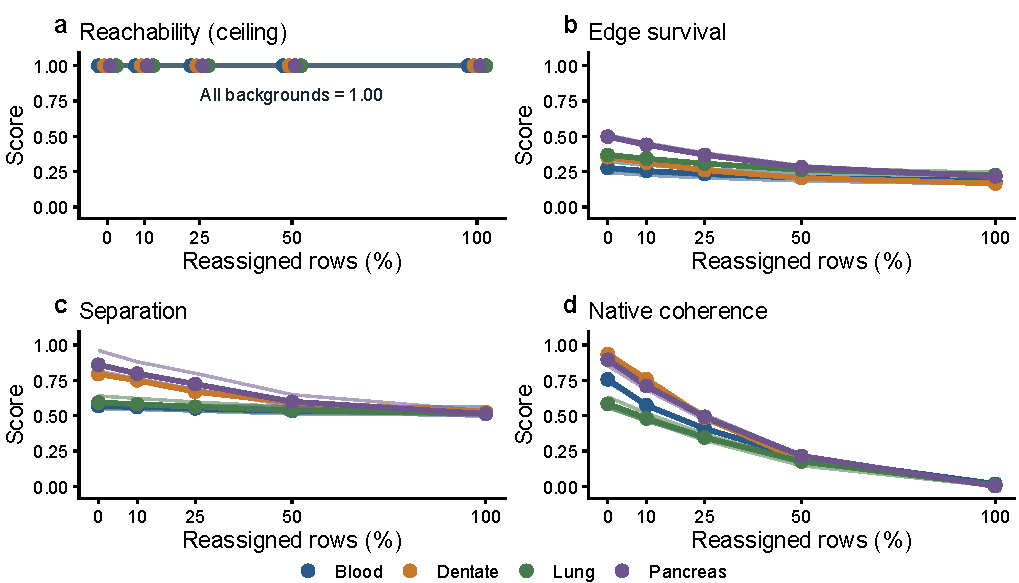
\includegraphics[width=\linewidth,height=0.64\textheight,keepaspectratio]{row_correspondence_sensitivity.pdf}
\caption{Sensitivity to disrupted cell correspondence at $k=15$ and 50 reference PCs. Panels A--D show reachability, edge survival, separation, and native allocation coherence, respectively. The single colour key between panel rows identifies the four backgrounds throughout the figure. Thick curves and points average three stored model seeds and three corruption seeds within each background; faint curves retain individual model seeds after averaging their three corruption seeds. The horizontal axis gives the selected row fraction at the five tested levels, 0, 10, 25, 50, and 100\%, rounded down to an integer cell count. Selected allocation rows are reassigned in one cycle, preserving their marginal distribution; each changes identity when at least two rows are selected. Repeated zero-fraction controls add no independent observations. Lines connect the tested fractions without fitting a response model. No error bars or population-level inference are implied, and the retained model-seed curves need not decline monotonically.}
\label{fig:correspondence}
\end{figure}

Forty-eight implementation controls rotate and uniformly rescale candidate coordinates or jointly reorder reference and candidate rows. Their largest absolute difference from the corresponding baseline, over the applicable geometry and coherence quantities, is $5.55\times10^{-16}$. Rotation is checked only for geometry because rotating a probability vector changes its allocation semantics. These controls support numerical invariance for the tested objects and software environment; they do not imply invariance to arbitrary reference changes.

The exact-tie stress test fails that invariance outside the stored population. The archived neighbour graph contains five self-loops for the twenty identical candidate rows. Joint row reordering changes edge survival by up to 0.0152 and separation by up to 0.1212 in absolute value, although reachability stays one. Duplicate coordinates make neighbour membership arbitrary, and positional self-removal is additionally unsafe. Thus an exactly collapsed representation needs an explicit identity-exclusion and tie policy before this implementation can support a permutation-invariant graph claim. The tie-free grid verification does not validate such an extension.

\FloatBarrier
\section{Discussion}

The experiments support a conditional interpretation of geometric fidelity: a score answers a question about specified inputs, graph settings, and annotations. Matching the starting noise changes the sign of a small local-score response to arm separation, while pair reachability still records substantial disconnection. Direct execution of the official trajectory API gives a strong shatter response that the local root-distance surrogate does not reproduce. These observations identify two distinct sources of misleading interpretation, experimental confounding and implementation misidentification. They also show why a calibration figure must preserve the actual coordinate intervention and why a metric name alone is insufficient evidence of what was computed.

The local and global diagnostics remain complementary after those corrections. Reachability is insensitive to a permutation of rows whenever the candidate graph remains connected, even though the correspondence to reference cells has been destroyed. The new corruption experiment demonstrates that limitation directly: mean reachability remains one, while mean edge survival decreases from 0.374 to 0.198 and native coherence from 0.793 to 0.009. A stable reachability value therefore cannot be interpreted as preservation of local identity. Conversely, a local score with a small response to a particular graph cut may still detect substantial noise or correspondence damage. The relevant comparison concerns response profiles under defined interventions.

The scale experiment further restricts how absolute values should be communicated. Across the tested neighbourhood sizes and retained reference dimensions, the median within-object range of edge survival is 0.312. Native coherence has a median range of 0.199. These changes arise without retraining or changing the candidate representation. They reflect a different measurement relation to the reference graph, and averaging them away would hide that dependence. The result favours reporting an explicitly chosen primary setting together with a sensitivity display. It does not identify an optimal neighbourhood size or establish that the setting with the highest score best represents the underlying biology.

The new paired differences show why a large absolute-score range need not imply that every ordering changes: edge difference signs persist in these twelve selected pairs, whereas separation has two setting-specific reversals and reachability is tied at baseline. Conversely, a stable descriptive edge sign is not evidence of model superiority because the paired objects differ in multiple features beyond the metric setting. The 999-draw results strengthen only the fixed-object correspondence check under the declared null; their identical minimum probabilities should not be read as twelve independent biological confirmations.

Exact coherence improves one narrower aspect of reproducibility. Its denominator is a property of all distinct allocation pairs and therefore does not depend on which row positions happened to enter a random sample. For the stored tie-free objects, joint-reordering controls differ by at most floating-point accumulation, and rotation with uniform rescaling preserves geometry scores. The exact-tie probe exposes a concrete exception: arbitrary neighbour membership and positional self-removal break the expected graph invariance under coordinate collapse. This numerical agreement therefore cannot be extended to arbitrary tie-breaking rules or representations. More fundamentally, an exact ratio can still describe a scientifically uninformative object. Eligibility must establish native probability semantics, and dispersion guards must accompany the ratio because nearly constant allocations provide little meaningful between-cell variation.

The stored-data census illustrates the importance of that eligibility denominator. Continuous coordinates, native allocations, guarded allocations, duplicate files, and repeated checkpoints all occur in the available collection. Counting them together would change the population being described and could create artificial precision. Our focused permutation comparison accordingly reports the eligible native population, while the full inventory retains every alias for provenance. Ten permutations yield a minimum possible Monte Carlo probability of one eleventh when the observed arrangement is included~\cite{phipson2010permutation}; an above-maximum count is therefore a descriptive comparison. Neither a large file count nor repeated optimizer seeds creates additional biological replication.

Several design choices remain limitations of this measurement study. The synthetic calibration uses a small planar branching fixture with coupled reference and faithful noise draws. Its discrete severities do not estimate a detection threshold or a power curve. The fixed real-data subset covers four backgrounds and three stored seeds per representation type, selected by configuration rather than outcome. Those objects are not a representative sample of all embedding algorithms, biological tissues, or training budgets. Their expression references preserve the historical transductive preprocessing and PCA fitting procedure. Consequently, the observed sensitivity cannot be interpreted as a test of generalization to cells excluded from every preprocessing step.

The practical implication is to make evaluation records more explicit. A reusable result should retain matched row identities, the reference construction, graph settings, the semantic type of the candidate, implementation versions, and unavailable or guarded outputs. The separate diagnostics then permit a reader to distinguish a loss of connectedness from local distortion, altered separation, or reduced allocation variation. Preserving those distinctions is also useful when a metric behaves unexpectedly: the investigator can revisit the responsible object or intervention instead of treating a composite score as a complete verdict. Our local source package includes the selected arrays and executable sensitivity analysis so that these relationships can be examined directly.

Biological validation remains an empirical next step with its own target. Count simulators such as Splatter~\cite{zappia2017splatter} and dynamic simulators such as dyngen~\cite{cannoodt2021dyngen} provide complementary settings for extending the planar fixture to more realistic expression and regulatory dynamics; neither was run here. Clonal lineage measurements, exemplified by transcriptional lineage tracing~\cite{weinreb2020lineage}, could then test whether a specified geometric property predicts observed fate rather than a computational annotation. Such evidence would also help choose a reference and a practically relevant effect size before testing a new representation. The present results establish neither those thresholds nor a universally preferred representation. They establish a more precise measurement contract, supported by noise-matched interventions, explicit allocation eligibility, exact denominator computation, and quantified sensitivity to graph scale and cell correspondence.

\section{Declarations}

\noindent\textbf{Data and code availability}\par\nobreak
The study-specific source repository is \url{https://github.com/PeterPonyu/reference-anchored-geometry}; the versioned research archive is \url{https://doi.org/10.5281/zenodo.22914409}. The archive contains the manuscript, seven vector figures, analysis code, synthetic calibration arrays, saved measurement tables, and 24 matched representation/reference arrays. It supports fixed-object sensitivity and permutation analyses and independent numerical checks. Complete historical expression caches, all inventoried latent files and the complete historical multi-library calibration driver are not supplied. The repository README gives the dependency requirements, commands and checksums. Source studies and their data-access conditions are identified in Materials and Methods and the bibliography. Author-owned software is MIT licensed; the author's manuscript, figures, generated results and weights are CC BY 4.0. Third-party data and annotations retain their original terms.

\noindent\textbf{Ethics approval and consent}\par\nobreak

This study analyzes synthetic fixtures and previously generated computational representations derived from public single-cell datasets. It involves no newly recruited participants, new animal experiments, or newly collected identifiable clinical records. The retained dataset accessions and source publications document the provenance of the original observations. The supplied study records contain no new ethics approval or participant-consent documentation for this secondary computational analysis; any institutional requirement must be assessed against that scope before submission.

\noindent\textbf{Funding}\par\nobreak

This research received no funding.

\noindent\textbf{Author contributions}\par\nobreak

Zeyu Fu is the sole author and was responsible for all aspects of the study and manuscript. Zeyu Fu is the corresponding contact for this manuscript.

\noindent\textbf{Competing interests}\par\nobreak
The author declares no competing interests.

{\small\setlength{\bibsep}{3pt plus 1pt minus 1pt}
\bibliographystyle{plainnat}
\bibliography{standalone-assets/refs,extra}}
\end{document}
